\documentclass[12pt]{article}
\usepackage[margin=1in]{geometry}
%\usepackage{hyperref}
\usepackage{amsmath}
\usepackage{graphicx}% http://ctan.org/pkg/graphicx
\usepackage{xcolor}
\usepackage{systeme}

%% Make red text
\newcommand{\com}[1]{\textcolor{red}{ #1}}



\usepackage[authoryear]{natbib}


\usepackage{tikz}
\tikzset{
  int/.style={circle, draw, fill=blue!20, minimum size=3em},
  init/.style={pin distance=1.2cm,pin edge={loop,thin,black}}
}
\usetikzlibrary{arrows}

\pagenumbering{arabic}

\newcommand{\XX}{21 } % number of methods
\newcommand{\rr}{\ensuremath{\mathcal{R}_0}}

\setlength{\itemsep}{0pt}





\begin{document}




\title{\XX dubious ways of estimating $\rr$}
\author{ Department of Statistics, Carnegie Mellon University}
\date{\today}
\maketitle

\tableofcontents

\section{Introduction}\label{sec:intro}
What has been called ``arguably the most important quantity in the study of epidemics'' \cite{Heesterbeek2002}, $\mathcal{R}_0$, the reproduction number, has been found to be an elusive quantity for epidemic modelers.  \citet{anderson1992} define $\rr$ as the ``the average number of secondary infections produced when one infected individual is introduced into a host population where everyone is susceptible.''  $\rr$, in some ways, summarizes an entire epidemic.  Despite the clear definition of $\rr$, epidemiologists have struggled to create a \textit{de facto} estimator for $\rr$  \citep{hethcote2000}.  The primary issue in estimating $\rr$ is that the quantity is a \textit{property of the model}, meaning that $\rr$ is dependent not only on the usual noise that comes with statistical modeling but also on a variety of assumptions on how we assume disease is transmitted through a population.

Typically, disease models are a part of the ``SI-framework'' pioneered by Kermack and McKendrick in the 1920s \citep{getz2006}.  Here, S and I are known as compartments where S stands for ``susceptible'' and I for ``infected.''  The issue arises in how individuals are assumed, either implicitly or explicitly, to travel from the S compartment to the I compartment and any other compartments that have been introduced such as immune, recovered, dead, or exposed, just to name a few.  One of the simplest models in the SI framework is the SIR model where R stands for a ``recovered'' state where individuals are no longer susceptible to the disease \citep{Kermack700}.  Even in this simplified framework, there is much dispute on how $\rr$ is to be estimated arising from assumptions on how populations intermix, if any intervention has been put in place, or whether disease parameters are constant over time.

Other issues of estimating $\rr$ include mathematical versus statistical approaches (i.e. solving for $\rr$ versus estimating $\rr$), how to estimate the quantity in the presence of different available data, and when to estimate $\rr$.  For instance, if only weekly incidence counts of a disease are available, then we have different methods of estimating $\rr$ than when we have more data available such as contact networks, the serial interval of a disease, and more.  Another major issue is that since $\rr$ is so difficult to estimate in the first place, the variance of the quantity has largely been glossed over or completely ignored.  This is especially troubling as we are concerned whether $\rr > 1$, which implies an outbreak of a disease.  A point estimate is simply not enough.

In short, $\rr$ is difficult to estimate because it is a property of the model.  This, in turn, makes it difficult to compare $\rr$ across different diseases or even instances of the same disease.  Many of these issues with estimating $\rr$ are summarized by \cite{li2011}

We review \XX ways to estimate $\rr$ over varying assumptions and in the presence of different sources of data.  The title of this manuscript is in reference to a seminal paper by Moler and Van Loan in 1978 (and its subsequent update in 2003) in which they calculate ``Nineteen dubious ways to compute the exponential of a matrix'' \citep{moler2003}.  We not only review the methods of estimating of $\rr$ but also include recommendations on when to use the methods as well as introducing techniques in which to estimate the variance of estimators.  We compare these estimates, when applicable, and find that $\rr$ is more robust than what was initially presumed.

The rest of this manuscript is organized as follows.  In Section \ref{sec:overview}, we introduce the methods in 3 broad groups:.  In Section \ref{sec:term} we introduce terminology used throughout.  In Section \ref{sec:details} we give an overview of each of the methods, what assumptions are used, what data is required, and where the method has been used in the past along with ways in which to calculate the variance for methods, when applicable.  In Section \ref{sec:results}, we give estimates of $\rr$ for the different methods and their variances over a variety of data sets.  Finally, in Section \ref{sec:dis} we discuss our conclusions and recommendations.


\section{Overview of \XX Methods to estimate $\rr$}
\label{sec:overview}

In order to organize the methods for estimating \rr, we have chosen four broad classes of estimation methods.  These partitions are meant to be guidelines of distinguishing methods from one another rather than immutable groups.  Many of these methods could have fit in another category or even all four of the classes chosen.  We have chosen the four classes as application of the survival function and its close relatives, classic compartment models, exponential growth assumptions, and estimation from networks.

\textbf{Point Estimation}
\begin{enumerate}
\item Survival function
  \begin{enumerate}
  \item Survival function (SF)
  \item Direct estimation of the survival function (DESF)
  \item Direct parameter estimation (DPE)

  \end{enumerate}
\item Compartment models 
  \begin{enumerate}
  \item SIR model
    \begin{itemize}
    \item Least Squares (SIR LS)
    \item Reparametrized Least Squares (SIR ReLS)
    \item Linear Model Approximation (SIR LMA)
    \item Linear Model Approximation, all time points (SIR LMAT)
    \item Max of Data (SIR Max)
    \item Smooth max (SIR SMax)
    \item Incidence-Prevalence Ratio (SIR IPR)
    \item Smooth Incidence-Prevalence Ratio (SIR SIPR)
    \item Harko's SIR model (HSIR)
    \item Attack rate (SIR AR)
    \item Sequential Bayes (SIR SB)
    \end{itemize}
  \item SEIR model (SEIR)
  \item Amplifier model (Amp)
  \item Next generation model (NGM)
  \end{enumerate}
\item Exponential growth 
  \begin{enumerate}
  \item Exponential growth (EG)
  \item Maximum likelihood of secondary infections (MLSI)
  \item Time dependent reproduction number (TDR)
  \item Initial growth rate and final size (IGRFS)
  \end{enumerate}
\item Estimation from networks 
  \begin{enumerate}
  \item Contact tracing (CT)
  \item Branching process (BP)
  \item Agent-based models (ABM)
  \end{enumerate}
  \end{enumerate}

  Additionally, we describe a number of variance estimates for the above methods for estimating \rr.  These are
  
\textbf{Variance Estimation}
\begin{enumerate}
\item Delta method
  \item Sensitivity analysis
  \end{enumerate}



\section{Epidemic Modeling Terminology}
\label{sec:term}

Here we introduce some of the terminology and notation used throughout the methods for estimating \rr.

{$\rr$} -- reproduction number -- 

{$\mathcal{R}_t$} -- effective reproduction number

{$\beta$} -- the infection rate

{$\gamma$} -- inverse of the expected recovery time

{$N_t$} -- Number of individuals in the population at time $t$

{$X(t)$} -- the number of susceptible individuals in a population at time $t$

{$Y(t)$} -- the number of infected individuals in a population at time $t$

{$Z(t)$} -- the number of recovered individuals in a population at time $t$

{$\omega$} -- serial or generation interval -- the time from onset of symptoms in an index case to the onset of symptoms in a subsequent case infected by the index patient

AR -- attack rate -- percentage of the population eventually infected



\section{Details for the \XX Methods}
\label{sec:details}
\subsection{Survival function}
\label{sec:direct}

The survival function is intimately with the theory of \rr, which originates from the field of demography in the late 1800s \citep{dietz1993estimation}.  Here, we have
\begin{align*}
\rr = \int_0^\infty p(a) \beta(a) da
\end{align*}
where $p(a)$ denotes the probability of a woman surviving age $a$ and $\beta(a)$ the rate of giving birth to a  girl for an individual of age $a$.  This interpretation also explains the name of \rr, which was imported to the field of epidemiology by MacDonald and Smith as reported by \cite{dietz1993estimation}.

This is the chronologically first and in many ways, the most direct method to calculate \rr.  However, this model also seems to be the most difficult to estimate.  We describe four methods attempting to estimate \rr from the survival function:  the survival function alone, direct estimation, and direct parameter estimation.


\subsubsection{Survival Function}
\label{sec:survival_fxn}
The first method, is not surprisingly, the survival function itself as presented by \cite{Heffernan2005}.  We change the notation from the above survival function to conform to the standards of epidemiology.  

Let $F(a)$ be the probability that a newly infected individual remains infectious for at least time $a$ (the survival probability,$p(a)$ in the previous definition).  Moreover, let $b(a)$ $(\beta (a)$ in the previous definition), the average number of newly infected individuals that an infectious individual will produce per unit time when infected for total time $a$.  Then $\rr$ is derived in Equation (\ref{eq:r0_survivalfxn}),

\begin{align}\label{eq:r0_survivalfxn}
  \rr = \int_0^\infty b(a)F(a)da.
\end{align}

This method presents one of the unique difficulties of estimating \rr: that of reconciling generations and time.  On the other hand, this method is flexible in that this derivation of $\rr$ is not restricted to compartment models.

Estimating this quantity in Equation \ref{eq:r0_survivalfxn} is hard and rarely attempted as $b(a)$ is particularly difficult to estimate, and it is due to this difficulty that the rest of these methods for estimating $\rr$ even exist.  

%%%%%%%

\subsubsection{Direct Estimation of the Survival Function }
\label{sec:direct-estim-surv}

\cite{fraser2004factors} have a derivation of $\rr$ related to the survival function based on the Van Forester equations,
\begin{align*}
  \frac{\partial Y(t, \tau)}{\partial t} +   \frac{\partial Y(t, \tau)}{\partial \tau} = 0,
\end{align*}
where $Y(t,\tau)$ is the number of people at time $t$ who were infected time $\tau$ ago.  $\rr$  is then,
\begin{align*}
\rr = \int_0^\infty \beta(\tau) d\tau,
\end{align*}
 where $\beta (\tau)$ represents the infectiousness at time $\tau$ since the infection.  Again, this model is more mathematical in nature than practical as $\beta (\tau)$ is difficult to estimate.


%%%%%%%%%%%%%%%


\subsubsection{Direct Parameter Estimation }
\label{sec:dpe}

This `plug and chug` approach as described by \cite{lipsitch2003} and \cite{dietz1993estimation} is the idea of estimating parameters $k$, the number of contacts per unit time, $b$, the probability of transmission per contact, and $D$ the mean duration of infectiousness to estimate $\rr$ directly from available data,
\begin{align}
\rr = kbD.
\end{align}

\cite{lipsitch2003} note that directly estimating $\rr$ in such a way may be difficult due to the available data.  They instead estimate $\rr$ using the mean serial interval, $\omega$, the time from onset of symptoms in an index case to the onset of symptoms in a subsequent case infected by the index patient in addition to the assumption of exponential growth of infected cases.

In the event, that the is estimate may be calculated, uncertainty estimates must be compounded, and to estimate $\rr$ alone, we only use data from the initial outbreak of the disease, so often we have a small sample size, resulting in large confidence sets.



\subsection{Compartment Models}
\label{sec:cms}

A large and the most common set of models used estimate $\mathcal{R}$ is that of compartment models (CMs).  As adapted from \cite{daley2001epidemic}, compartment models consist of the following.  CMs model how objects move from one discrete state to another over time and provide a high-level model of how diseases, for instance, may be spread throughout a population.  Within the CM framework, we make four essential assumptions,
\begin{enumerate}
\item The compartments are discrete and have no overlap.
\item The transition of objects among compartments is described by a set of equations.
\item The populations mix homogeneously
  \item The number of objects in each compartment at time $t=0$ is known
  \end{enumerate}  


Another common assumption for compartment models, is the law of mass action, a property borrowed from chemistry which says that the mass of the product is proportional to the mass of the reactants.  \cite{anderson1992} adapt the law of mass action to epidemiology saying, ``the net rate of spread of infection is assumed to be proportional to the product of the susceptible people times the density of the infectious individuals.''  Therefore, the flow of objects from one compartment to another may be dependent on the percentage of objects within one or many of the compartments.  The assumption of mass action holds particularly true for disease modelling as typically we assume infections at the next state are proportional to both the susceptible and infected populations at the current state.

For disease modelling, all CMs fall into the SI-framework, meaning that there is a susceptible population that may become infected.  Thus, we require there be susceptible and infected compartments but also allow additional compartments such as the recovered state, an exposed latent state, and more.  CMs may either work with continuous or discrete time and \cite{getz2006} remark that there is no preference between the two.

In this section, we discuss 14 different CMs used to estimate $\mathcal{R}$.  Different CMs yield different mathematical derivations of \rr.  That is, for example, an SIR model with non-constant population will yield a different mathematical formula for \rr than the SEIR model with non-constant population.  The only difference in these two models is that the SEIR model.  That said, even within the same compartment model framework, we can estimate \rr in a variety of ways.  In fact, we describe 11 methods to estimate \rr, within the SIR framework!  Most of these methods are descriptions to estimate parameters within the SIR model and may be extended to other CM frameworks such as the SEIR model.  The final method described in this section, the next generation operator (NGM) is a general method to derive \rr from almost any CM.




\subsubsection{SIR Model}
\label{sec:sir-model}

We begin with the most popular CM, the SIR model.   First introduced to epidemiology by  \cite{Kermack700}, the SIR model governs how individuals transition from \textbf{S}usceptible, \textbf{I}nfected, and \textbf{R}ecovered compartments.  The model is represented graphically in Figure \ref{fig::sir}.  In this model, once a person is recovered she cannot have the disease again.

\begin{figure}[h]
\centering
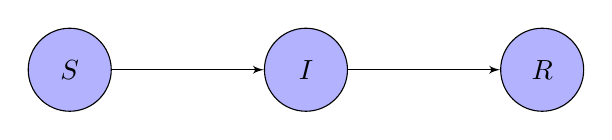
\begin{tikzpicture}[node distance=3cm,auto,>=latex',every node/.append style={align=center}]
    \node [int,  fill = white!70!blue] (a)              {$S$};
    \node [int,  fill = white!70!blue]           (c) [right of=a] {$I$};
    \node [int,  fill = white!70!blue] (e) [right of=c] {$R$};
    \path[->, auto=false] (a) edge node {} (c)
                          (c) edge node {} (e) ;

\end{tikzpicture}
\caption{Depiction of a SIR model.  One can only get the disease once in this model.}\label{fig::sir}
\end{figure}
Here, $N$ is the number of individuals in the system.  As we see no arrows pointing out of the nodes in Figure \ref{fig::sir}, then $N$ is constant throughout time.  Simple adaptations of the SIR model can include birth and death rates, which will correspondingly change the derivation of $\rr$ (for more information, see Section \ref{sec:ngm}). The parameters  $\beta$ and $\gamma$ have epidemiological meaning.  Here, $\beta$ is the average infection rate and $\gamma$ is the inverse of the average recovery rate.  The model is represented through the ODEs in Equation \ref{eq::sir}.  Throughout, we use $X$, $Y$, and $Z$ for stand-ins for the ODEs for $S$, $I$, and $R$, respectively to avoid confusion.
\begin{align}
\systeme{\frac{dX}{dt} = -\frac{\beta XY}{N}, \frac{dY}{dt} = \frac{\beta XY}{N} - \gamma Y, \frac{dZ}{dt} = \gamma Z}. \label{eq::sir}
\end{align}

In words, susceptible individuals become infected at a rate that is proportional to the proportion of infected people multiplied by $\beta$, the infection rate, and the number of susceptible individuals.  Infected individuals recover at a rate of $\gamma$ multiplied by the number of infected individuals.

An epidemic occurs if 
\begin{align*}
  \frac{dY}{dt} &> 0 \\
\frac{\beta S I}{N}  - \gamma I &> 0 ,
\end{align*}

that is,  the rate of new infections is greater than the rate of recovery.  So as long as $\frac{S}{N} \approx 1$ then an epidemic will occur if
\begin{align}\label{eq:sir_r0}
  \rr = \frac{\beta}{\gamma} > 1.
  \end{align}

In the ideal set up, we have data of the number of Susceptibles, Infectious, and Recovered individuals at different points over time.  From this we would like to estimate the $\beta$ and $\gamma$ parameters and ultimately $\rr$.

There are numerous ways to estimate the parameters in this model.  We detail 11 of them here.

\subsubsection{Least Squares ($\beta$, $\gamma$) (SIR LS)}\label{least-squares-beta-gamma}

We find

\begin{align*}
(\hat{\beta}, \hat{\gamma} )&=\text{argmin}_{\beta, \gamma} \sum_{t} (Y(t)_{obs} - Y(t))^2 
\end{align*}

Then \(\hat{R}_0= \frac{\hat{\beta}}{\hat{\gamma}}\).

We can use gradient descent or another solver to find estimates for these parameters.  If we assume $Y= f(t) + \epsilon_t$ with $\epsilon_t \overset{iid}{\sim} N(0, \sigma^2)$ where $f(t) = \int_0^t \frac{dY}{dt} dt$, then this this method is equivalent to finding the MLE of $\beta$ and $\gamma$.  However, we note that the assumption of homoskedasticity seems likely to be violated in this model.

\subsubsection{Reparametrized Least Squares ($\rr$, $\gamma$) ( SIR ReLS)}\label{reparametrized-least-squares-rux5f0-gamma}

We reparametrized the the ODES in Equation \eqref{eq::sir} directly with \(\rr\) and \(\gamma\), using the relation $\rr = \frac{\beta}{\gamma}$.

\begin{align*}
  \left \{
  \begin{array}{cl}
    \dot{X} &= - \rr \gamma Y \frac{X}{N}\\
    \dot{Y} &=  \rr \gamma Y \frac{X}{N}  - \gamma Y \\
    \dot{Z} &=  - \gamma Y 
  \end{array}
  \right .
  \end{align*}

We find

\begin{align*}
(\hat{R}_0, \hat{\gamma} )&=\text{argmin}_{\rr, \gamma} \sum_{t} (Y(t)_{obs} - Y(t))^2 .
\end{align*}

We use the \(\rr\) directly from the above calculation.

\subsubsection{Linear Model Approximation (SIR LMA)}\label{linear-model-approximation-degree-10}

The idea that an SIR model may be well approximated by a linear model is described by \cite{chang2017}.  We borrow this idea here and use the ODES in Equation \eqref{eq::sir} to relate our estimated linear model to that of $\rr$.

Specifically, we fit a linear polynomial of \(t\) with degree \(K= 10\) model to \(X\)
and \(Y\) using least squares to find the coefficients (\(\hat{x}_k\),
\(\hat{y}_k\)),

\begin{align*}
X(t) &= \sum_{k=0}^K x_k t^k\\
{Y}(t) &= \sum_{k=0}^K y_k t^k
\end{align*}

Then, we estimate the derivatives as

\begin{align*}
\hat{X}^\prime(t) &= \sum_{k=1}^K k \hat{x}_k t^{k-1}\\
\hat{Y}^\prime(t) &= \sum_{k=0}^K k \hat{y}_k t^{k-1}
\end{align*}

Then \(\rr\) is calculated as according to the ODES,
\[\rr = \frac{\hat{X}^\prime(0)}{ \hat{X}^\prime(0) + \hat{Y}^\prime(0)} \cdot \frac{N}{X(0)} \]

Like in the previous cases, we are assuming the true models are

\begin{align*}
X(t) &= \sum_{k=0}^K x_k t^k + \epsilon_t\\
  {Y}(t) &= \sum_{k=0}^K y_k t^k + \epsilon_t,
\end{align*}
with $\epsilon_t \overset{iid}{\sim} N(0, \sigma^2)$.  Here, $K=10$ is rather arbitrary and should be selected using some criterion such as AIC in addition with the knowledge of how many data points are available to the user.

\subsubsection{Linear Model Approximation, All Time Points (SIR LMAT)}\label{linear-model-approximation-all-time-points-degree-10}

We fit a linear polynomial of \(t\) with degree \(K= 10\) model to \(X\)
and \(Y\) as above, with a slight modification in how we calculate
\(\rr\),
\[\rr = \frac{1}{\# \text{ Obs}}\sum_t \frac{\hat{X}^\prime(t)}{ \hat{X}^\prime(t) + \hat{Y}^\prime(t)} \cdot \frac{N}{X(0)} \]
The idea is that $\frac{\mathcal{X}^\prime}{X^\prime + Y^\prime}$ is constant in $t$, but due to our approximations with the linear model, this is no longer the case.  Here, we average over the different possible values of $\rr(t)$.

\subsubsection{Max of Data (SIR Max)}\label{max-of-data}

Under the SIR model there is an absolute maximum of infected individuals $Y$.  We note that \(Y^\prime(t) = \frac{\beta XY}{N} - \gamma Y > 0\) when \(\rr = \frac{\beta}{\gamma} < \frac{X(t)}{N}\). The max
of \(Y\) occurs when \(Y^\prime = 0\) and hence
\[\rr = \frac{N}{X_{obs}(t^*)},\] where
\(t^* = \text{arg max}_{t} Y_{obs}(t)\).  

\subsubsection{Smooth Maximum of Data (SIR SMax)}\label{smooth-maximum-of-data}

We use a spline with 4 degrees of freedom to fit both \(X\), and \(Y\).
We then apply the principle as above, except now,
\[\rr = \frac{N}{\hat{X}(t^*)},\] where
\(t^* = \text{arg max}_{t} \hat{Y}(t)\). 

\subsubsection{Incidence to Prevalence
Ratio (SIR IPR)}\label{incidence-to-prevalence-ratio}
In terms of data from the SIR model, incidence $J(t) \approx -(X(t+1) - X(t))$, and the IPR$(t) = \frac{J(t)}{Y(t)}$. The actual reproduction number, $R_a(t) = \text{IPR}(t)\cdot D$ where $D = 1 /\gamma$.  This method assumes that we have some prior knowledge about $\gamma$.  Thus we use as our estimate,
\begin{align*}
\rr &= R_a(0).
\end{align*}

Here we assume that the time step is small enough to approximate the incidence.

\subsubsection{Smoothed Incidence to Prevalence Ratio (SIR SIPR)}
We use the same method as above, but first fit splines with 4 degrees of freedom, $\hat{X}(t)$ and $\hat{Y}(t)$, , to fit to $X_{obs}$ and $Y_{obs}$, respectively.  Then  $J(t) \approx -(\hat{X}(t+1) - \hat{X}(t))$, and the IPR$(t) = \frac{J(t)}{\hat{Y}(t)}$.  Then
\begin{align*}
\rr &= R_a(0).
\end{align*}

%%%%%%%%%%%%%%%%%%%%%
\subsubsection{Harko (HSIR)}
Recently, \citep{harko2014exact} were able to reduce the SIR equation, with the following set of ODEs (reparametrized from Equation \eqref{eq::sir})

\begin{align*}
  \left \{ \begin{array}{ll}
             \frac{dX}{dt} &= - b X(t) Y(t) \\
             \frac{dY}{dt} &=  b X(t) Y(t) - \gamma Y\\
             \frac{dZ}{dt} &= \gamma Y,\\
           \end{array}
  \right .
\end{align*}

where $b = \frac{\beta}{N}$, to one differential equation.  Here,
\begin{align*}
  u(t) &= e^{\frac{\beta}{\gamma}Z} \\
  t - t_0 &= \int_{u_0}^u \frac{d \xi}{\xi (C_1 - \gamma \log \xi + X(0) b \xi)},
\end{align*}
where $C_1 = -\frac{b}{N}$.  Then

\begin{align}
  X &= X(0) u  = X(0) e^{\frac{\beta}{\gamma}Z} \nonumber\\
  \log \frac{X(t)}{X(0)} &=  \frac{b}{\gamma}Z =  \frac{\beta}{\gamma N} Z \nonumber\\
  \log \frac{X(t)}{X(0)} &=  \frac{\rr}{N} Z \label{eq:harko_lin}
\end{align}

If we add error into Equation (\ref{eq:harko_lin}), then we have

\begin{align}
  \log \frac{X(t)}{X(0)} &=  \frac{\rr}{N} Z  + \epsilon_t\label{eq:r0_harko}
\end{align}

If we assume $\epsilon_t \overset{iid}{\sim}N(0, \sigma^2)$, then we can directly estimate $\rr/N$ through linear regression and also an expression for the variance.  This method greatly simplifies the computational effort needed to estimate $\rr$ as it does not require any numerical integration.

\subsubsection{Attack Rate (SIR AR)}

The Attack Rate (AR) as described by \cite{obadia2012r0} as the ``percentage of the population eventually infected.''  Under the SIR (XYZ) model with constant population,

\begin{align}\label{r0_attackrate}
\rr =  \frac{\log \left (\frac{1  - AR}{X(0)/N}  \right ) }{AR - (1 - X(0)/N)}
\end{align}

This method can only be used to assess $\rr$ after a disease has passed through a population.  Additionally, if either $\beta$ or $\gamma$ were affected during the disease's lifetime then $\rr$ cannot be properly assessed.


\subsubsection{Sequential Bayes (SIR SB)}\label{sec:seqbayes}

Posited by \cite{bettencourt2008} and summarized in \cite{obadia2012r0}, this method uses a Bayesian approach to an approximation to the classic SIR model.  The approximated SIR model is that the incidence at $t+1$, $N(t+1)$ is from a Poisson distribution, with $\gamma$ as the  average inverse of the infectious period and $R$ as the effective reproduction number, which we take here to be $\rr$.

In order to estimate $\rr$, we must have some idea about the serial interval, $\omega$.
\begin{align*}
N(t+1)  \sim Poisson( N(t) \exp \left \{  \gamma (R-1)\right \})
\end{align*}
Then, the posterior distribution of $\rr$ given the previous days' incidences is
\begin{align*}
  P(\rr | N_0, \dots, N_{t+1}) = \frac{P(N_{t+1} | \rr, N_0, \dots, N_t)P(\rr| N_0, \dots, N_t)}{P(N_0, \dots, N_{t+1})}.
\end{align*}
This method is sequential in that the prior distribution for $\rr$ comes from the previous day.  The initial prior for $\rr$ is assumed to be flat.  This method results in a posterior distribution from which credible intervals may be obtained.  This method assumes, initial growth in incidence to be exponential, and homogeneous mixing of populations as with any compartment model.




\subsubsection{SEIR Model (SEIR)}
\label{sec:seir-model}

The SEIR model is a common adaptation of the SIR compartment model \com{add references that use this method}.  The ``E'' compartment stands for ``exposed'' and represents the stage where individuals are infected but not yet infectious.  The model is described by the following set of equations, as described by \cite{cintronarias2009}.  This particular model here does not include birth and death rates but the model can be adapted to do so,
\begin{align*}
  \frac{dX}{dt} &= - \frac{\beta XY}{N} \\
  \frac{dE}{dt} &= \frac{\beta XY}{N}  - \alpha E\\
  \frac{dY}{dt} &= \alpha E - \gamma Y \\
  \frac{dZ}{dt} &= \gamma Y.
\end{align*}

Then $\rr = \beta / \gamma$, just as in the SIR model.  As in the SIR model, $\beta$ and $\gamma$ have the same interpretation and $\alpha$  The methods used to estimate the parameters $\beta$ and $\gamma$ are of the same class used to estimate those parameters in the SIR model.  The important difference between this method and the SIR model is the assumption of a 4th class, the exposed compartment.  Even though the derivation for $\rr$ is the same for both the SIR and SEIR model, this will still result in different results for estimations of \rr, even if the same method for estimation of parameters is used.  Typically, some form of least squares is used to estimate parameters in this model. We demonstrate this in Section \com{results}.





\subsubsection{Amplifier Model (Amp)}
\cite{blower2004} discuss the case where a disease may have different strains and consequently different reproduction numbers.  They introduce a multistrain mathematical model called the amplifier model to deal with this case.

This model is based on the the SLIR compartment model, where $L$ stands for latently infected individuals and $T$ for diseased individuals.  There is a set of ODEs for each strain of the disease with different parameters for recovery, transmission rate, and drug resistance of the disease.  Additionally, there is mixing of the different strains as ``the amplifier model also allows for immigrating and emigration of individuals of all types, as well as reinfection of latently infected individuals'' \citep{blower2004}.  The details may be found in their manuscript.  Ultimately, their derivation for $\rr^{(i)}$ where $i$ stands for the $i$th strain is
\begin{align*}
\rr^{(i)} = X^* \frac{ ( \beta_i^T + \beta_i^L)\nu_i + \beta_i^T \mu_i^L}{(\nu_i + \mu_i^L)(c_i + k_{i,i+1} + \mu_i^T)}.
\end{align*}
Here, $X^*$ is the number of susceptibles individuals in the disease-free equilibrium in the absence of immigration or emigration; $\beta_i^L$ and $\beta_i^T$ are strain-specific transmission rates for the latent, and infected classes, respectively; $\nu_i$ denotes the progression rate from latently infected to disease for strain $i$; $\mu_i^L$ and $\mu_i^{T}$ are death rates for the latent and infected classes, respectively; $c_i$ is the cure rate; and $k_{i, i+1}$ is a parameter associated with the degree of amplification of drug resistance.  They note that ``each reproduction number is the product of average number of secondary infections caused per unit time, the aver time a case remains infectious and the probability that an infected individual develops disease.''

In the amplifier model, $\rr$ was derived from using the stability point (disease free equilibrium state in the absence of immigration or emigration) of the system by solving the characteristic polynomial for the eigenvalues.  This derivation is explained in more depth in Section \ref{sec:ngm}.

We show this model as opposed to other available CMs because it shows not only how complicated CMs can become, but researchers approach the assumption of homogeneity, which is often suspect.  In this case, we have strain-specific transmission rates, so we are essentially stratifying compartments into different sets.  Very complicated models have arisen from stratification of compartments, which leads to the approach of ABMs.


\subsubsection{Next Generation Model (NGM)}
\label{sec:ngm}

The Next Generation Model (NGM) is a generalization of any compartment model at the infection-free steady state. This model solves the problem of having an expression of $\rr$ in terms of the epidemiological parameters for a general compartment model.  Originally, introduced by \citep{diekmann1990}, \cite{diekmann2009} posit a recipe to find $\rr$ for a wide class of compartment models, including commonly used ones such as MSEIR, MSEIRS, SEIR, SEIRS, SIR, SIRS, SEI, SEIS, SI, and SIS \citep{hethcote2000}. We summarize that recipe here, using their notation.  First, define the \textit{infected subsystem} as ``the equations of the ODE system that describe the production of new infections and changes in state among infected individuals.''  Let $x = (C_1, C_2, \dots, C_m)$ where $C_i$ are the different compartments of the infected subsystem.  The steps to find $\rr$ are as follows:


\begin{enumerate}
\item ``Linearize the infected subsystem of nonlinear ODEs about the infection-free steady state''
\item Decompose the linearized infected subsystem into $(T + \Sigma )x$ where $T$ is a $m\times m$ matrix of transmissions and $\Sigma$ is a $m \times m$ matrix of transitions.
\item $\rr$ is the spectral radius (i.e. the dominant eigenvalue) of $K_L=-T \Sigma^{-1}$.  Here $L$ stands for the ``large domain.''
\end{enumerate}

Here, $T_{ij}$ is the rate of transmission of \textit{newly} infected individuals in state $i$ created by individuals in state $j$.  $\Sigma_{ij}$ is the transition rate of individuals into compartment $i$ from compartment $j$.

This method has the assumptions of a basic compartment model: homogeneous mixing among populations and the law of mass action, i.e., that the number of infected individuals are proportional to the number of infected individuals at the previous step.  The estimations for $\rr$ from the previously mentioned compartment models may also be derived using this method.  Additionally, this method is advantageous in that the matrix $\Sigma$ has an intuitive meaning.

Although, this method is useful for deriving an expression of $\rr$, it is unclear how to actually estimate it from these expressions.  Again, least squares is typically used to estimate such parameters.

%%%%%%%%%%%%%%%%%%%%%%%%

\subsection{Exponential Growth}\label{sec:exp-growth}
Typically, CMs expressed through differential equations have no known analytical solutions, which makes deriving an expression for $\rr$ difficult.  One simplification that is often introduced to the SI framework is that of exponential growth, or that the number of infections in the beginning of an epidemic mimics that of an exponential curve.  This simplified expression has allowed for many derivations of $\rr$.


\subsubsection{Exponential Growth (EG)}
\label{sec:expgrowth}
\cite{wallinga2007generation} report that $\mathcal{R}_t$ and hence $\rr$ may calculated by using the fact that infection ``counts increase exponentially in the initial phase of an epidemic.''  We need to know $r$, the \textit{per capita} change in the number of new cases per unit of time and $\omega$ the serial interval.

Then, we have

\begin{align}\label{eq:lotka}
\rr = \exp{(r \omega)}
\end{align}
or its first order approximation

\begin{align}\label{eq:anderson}
\rr = 1 + r \omega.
\end{align}


Equation \eqref{eq:lotka} is derived from a demographic view using the Lotka-Euler survival equations which come from the fields of demography, ecology, and evolutionary biology, whereas Equation \eqref{eq:anderson}is derived through an epidemiologist.  These estimates for $\rr$ between Equation \eqref{eq:lotka} and Equation \eqref{eq:anderson} can be strikingly different.

\cite{wallinga2007generation}, instead, use a moment generating function expression for $\rr$.  With $g(a)$ as the distribution of age at infection, then

\begin{align*}
\rr^{-1} &= \int_{a=0}^\infty e^{-ra}g(a)da.
\end{align*}

For all these above estimations of $\rr$, we observe the duration of serial intervals in a period of exponential growth.  Deciding when this occurs and which data to use to estimate $\rr$ is difficult.  \citeauthor{wallinga2007generation} specify $\omega$ in multiple ways.  Parametrically, they use exponential, normal, and delta distributions.  They also observe the empirical distribution of the serial interval.

\citeauthor{wallinga2007generation} note that specifying the epidemic model ``implicitly specifies a generation interval distribution.''  The above equations are under the SIR framework, but this method may be adapted to acommodate frameworks such as the SEIR model and more.

\subsubsection{Maximum Likelihood Estimator of Secondary Infections (MLSI)}\label{sec:mle-si}
This method, described by \cite{forsberg2008}, finds the estimate of $\rr$ by maximizing the likelihood function under certain assumptions.  We assume that the ``the number of secondary cases produced by an infected individual follows a Poisson distribution, and that the serial interval is described by a multinomial distribution.''  Recall, the serial interval is the distribution of time between a primary case developing symptoms and a case infected by the primary case developing symptoms.  An approximate version of this can be simplified to a thinned Poisson in Equation \ref{eq:mlesi} where
\begin{align}\label{eq:mlesi}
  L(\rr, \mathbf{p}) = \prod_{t=1}^T \frac{e^{- \rr \sum_{j=1}^{\min(k,t)}N_{t-j}p_j}\left (\rr \sum_{j=1}^{\min(k,t)}N_{t-j}p_j \right )^{N_t}}{N_t!}.
\end{align}
Here, $k$ is the maximal amount of the serial number, $T$ is the total time and $p_j$ is the probability of displaying symptoms on day $j$ after being infected.  The number of cases on day $t$, $N_t$ are incidence counts that are known. 

This method assumes a Poisson distribution on $\rr$ in addition to assuming a multinomial on the serial interval.  Additionally, this method also assumes a period of exponential growth,


%%%%%%%%%%%%% 5

\subsubsection{Time Dependent Reproduction Number (TDR)}\label{sec:timedep}
This is another method used to estimate the effective reproduction number, which again, we take to be $\rr$ here \citep{forsberg2008}.  This is a likelihood based approach where we maximize the likelihood that case $i$ has been infected by case $j$ at certain time using the serial interval, $w(t)$ where $t_i$ is when case $i$ was infected and $N$ is the total number of cases,
\begin{align*}
  p_{ij} &= w(t_i- t_j) / \sum_{i \neq k} w(t_i - t_k),\\
  \rr &= \frac{1}{I(0)}\sum_{i=1}^N p_{i0}
  \end{align*}

  It is assumed we have some idea about the generation interval distribution, $w(t)$.

\subsubsection{Initial Growth Rate and Final Size (IGRFS)}
\label{sec:igr-fs}

Initial growth rate, as described by \cite{dietz1993estimation} is derived by \cite{anderson1986}, initially to study the spread of HIV estimates $\rr$ through
\begin{align*}
\rr = \frac{D \ln 2} {t_d} + 1,
  \end{align*}
  with $D$ as the average incubation period and $t_d$ as the doubling time during its early stages.  This method assumes you know when the ``early stage'' ends along with knowledge of the average incubation period.  

  Final size, on the other hand, only looks at $\rr$ once a disease has run its course.  Here $\mu_0$ is the proportion of initially infected individuals and $\mu_\infty$ is the final, cumulative proportion of infected cases at the end of an epidemic,
  \begin{align*}
    \rr = (1- \mu_\infty)^{-1} \ln \mu_\infty^{-1}.
  \end{align*}

  For final size, it is assumed the initial population is completely susceptible

  These two methods allow one to look at $\rr$ at both the beginning and the end of an epidemic.  However, both approaches have advantages and disadvantages.  For the initial growth rate, while one can see $\rr$ at early stages, estimating the doubling time $t_d$ is difficult.  For final size, one has to wait until the end of an epidemic to calculate $\rr$, and preventions of the disease may skew the final result.
%%%%%%%%%%%%%%%%%%%%%%%%%%%%%%

  \subsection{Estimation from Networks}
As estimating $\rr$ is concerned with the number of new infections based on the contacts of old infections, a network is a seemingly intuitive way to model such contacts and hence infections.  Networks that have been used to estimate $\rr$ include contact tracing of actual individuals, branching processes to model the spread of disease, and agent-based models (also known as individual level models), which all leverage networks along with different sources of data to generate estimates of $\rr$.
  
\label{sec:network}

%%%%%%%% 5
\subsubsection{Contact Tracing (CT)}
\label{sec:contact_tracing}
A reasonable idea to estimate $\rr$ is to directly observe the number of secondary infections produced by an initial infector.  However, this approach is generally impractical as it is difficult to estimate every single contact a person may have.   With seriological information, we could conceivably recreate the transmission of the disease throughout a population.  Even in this case, it is unlikely, for one, to have a completely susceptible population, which is essential to an unbiased estimate of $\rr$.  Moreover, this would implicitly be conditioning on the initial infector's contacts which may not reflect those of the rest of the population.  We write the calculation for $\rr$ under contact tracing in Equation \ref{eq:r0_contacttracing}, where $X_0$ is a random variable denoting the number of individuals in the population person 0 infects.  Here $S_0=N$ indicates that the initial number of susceptibles is $N$, the size of the population.

\begin{align}\label{eq:r0_contacttracing}
\rr = E[ X_0 | S_0 = N]
\end{align}

\cite{eames2003} describe contact tracing as an ``extreme form of targeted control, where the potential next-generation cases are the primary focus,'' that is, one focuses on treating the contacts of an infected individual rather than applying uniform treatment across a population.  They note that this method has ``proved to be a highly successful strategy when the number of infectious cases is low'' and ``is the standard tool for eliminating minor outbreaks in the latter stages of disease eradication.''

They describe an estimate for $\rr$ for a SIR model on a network, with $r$ as the rate of transmission across a contact multiplied by the infectious period and $n$ as the number of contacts as

\begin{align*}
\rr = r(n-2)
\end{align*}


%%%%%%%%%%%%%%%%%%%%%%%%%%%%%%%%

\subsubsection{Branching Process (BP)}
\label{sec:branching-process}

Branching processes are models for population growth which track generations of new offspring.  We describe branching processes as adapted for epidemic modelling from the notation of \cite{grimmett1991}.  An infector $i$ may produce new infections, called offspring, over the lifetime of the  infector $i$'s disease.  The offspring of the original infector directly produces are called the first generation.  The offspring of the first generation are called the second generation and so on.  An important assumption in branching processes is that the offspring produced from different infectors are indepedent and identically distributed, and so for a branching process to be a valid model in epidemic modeling, we must assume a large population with few infectors.

\com{draw a family tree}

\cite{getz2006} give a way to calculate $\rr$ from a branching process.  ```We define the offspring distribution $\{q_i \}_{i=0}^\infty$, where $q_i$  is the probability that an infectious individual infects $i$ other individuals.  Thus we require $\sum_{i=0}^\infty q_i =1$ and note that $\rr$, the mean number of cases contracting disease from each infective'', is simply given by'
  \begin{align*}
    \rr = \sum_{i=0}^\infty iq_i.
  \end{align*}
  It is assumed we know how to estimate the $q_i$, and so in this case, it is not too different of an approach than contact tracing.


    

\subsubsection{Agent-Based Models (ABM)}
\label{sec:agent-based-models}
Agent-based models (ABMs) or individual level models (ILMs) are ``bottom-up'' models, meaning micro patterns are simulated and macro patterns are then derived from these simulations.  ABMs consist of agents which represent individuals (e.g., people, mosquitoes, poultry) and a series of activities in which the agents can affect one another and evolve over time.

In epidemiology, ABMs can be used to simulate the spread of disease.  ABMs allow for every detail of an infection to be known, in the context of estimating $\rr$, meaning we know exactly who is infected by whom and when.  Thus $\rr$ can be calculated simply through
\begin{align*}
  \rr = \frac{1}{\# \text{ simulations}}\frac{1}{\#\text{ initial infections}} \sum_{(s \in \text{ simulations})}\sum_{(i \text{ infected at } t=0)} \# \text{ infected by $i$ in simulation }s.
\end{align*}

The difficulty in the ABM lies in calibrating the evolving of agents over time to accurately reflect reality, which is a problem that cannot be understated.  Thus, it is typically necessary to have knowledge of parameters such as the serial interval, transmission rate, recovery rate, etc.  Additionally, we need to have accurate agents in number, characteristics, and their implied network structure.  ABMs are flexible in that they may be used with any model in the SI framework.  The only requirement is that we track who infects whom and can adapt for any additional states such as exposure.

Examples of calculations of $\rr$ using ABMs/ILMs are in \cite{breban2007,ahmed2013variance}.





\subsection{Variance Methods}
\label{sec:methods}

Estimating $\rr$ is difficult, and it is no different for estimating $V[\rr]$, the variance.  We describe four general methods which may be applicable to estimate the variance.  We describe the assumptions that are used along with each method and note that they may not be applicable to all of our methods.  Still, reporting confidence intervals, or at the very least, standard deviations is very important and we hope to encourage this practice by describing the below methods used to estimate models in the SIR framework in a simple fashion.


\subsubsection{Delta Method}\label{delta-method}

When the method estimates \(\beta\) and \(\gamma\) instead of \(\rr\) directly, we use the delta method approximation to calculate the
variance of \(\rr\). Here, we know \(\rr = h(\beta, \gamma) = \frac{\beta}{\gamma}\). Then \(\bigtriangleup h = (\frac{1}{\gamma},  -\frac{\beta}{\gamma^2})^T\).  Then \(V[\rr] = \bigtriangleup h^T \Sigma_{\beta, \gamma} \bigtriangleup h\), where \(\Sigma_{\beta, \gamma}\) is covariance matrix of \(\beta\) and \(\gamma\).

This estimate assumes that the distribution of $\beta$ and $\gamma$ are asymptotically normal.  Here, we use the relationship of $\rr = \frac{\beta}{\gamma}$ in order to estimate the variance, which is specific to the SIR framework.  This method may be extended to other frameworks and we provide some examples here \com{add examples of SEIR, serial interval, etc.}

\subsubsection{Sensitivity Analysis}\label{sensitivity-analysis}

We estimate \(\frac{\partial Y}{\partial \beta}\) (or
\(\frac{\partial Y}{\partial \rr}\) when using reparametrized least squares) and \(\frac{\partial Y}{\partial \gamma}\) at each time point \(t\) using the estimated \(\beta\) or \(\gamma\) from the estimation process where $Y$ stands for the number of infected at time $t$. Then an approximation of the covariance matrix is \((\chi^T \chi)^{-1}\) where \(\chi_{ij} = \frac{ \partial Y(t_i)}{ \partial \theta_j}\) where \(\theta\) is a vector of parameters. \com{add citation}



%%%%%%%%%%%%%%%




\section{Analysis and Results}
\label{sec:results}

\section{Discussion}
\label{sec:dis}


\label{sec:details}




\bibliographystyle{apa}%Choose a bibliograhpic style
\bibliography{Master}




\end{document}


%%%%%%%%%%%%%%%%%%%%%%
\Textbf{Title:} 

\textbf{Author:} 

\textbf{Citation:} 

\textbf{Major themes:} 

\textbf{Notes:}
\\
%%%%%%%%%%%%%%%%%%%%%%




\begin{figure}[h]
\begin{center}
\includegraphics[width=4in]{mvhw7_3c.pdf}
\end{center}
\caption{
Biplots of the different continuous variables and their correlations.}\label{fig3c}
\end{figure}

%% two pictures whoa

\begin{figure}[h]
\centering


\begin{figure}[h]
\centering

\begin{subfigure}{.5\textwidth}
  \centering
  \includegraphics[width=1\linewidth]{mt_eda_cont_hists.pdf}
  \caption{Histograms of Arrival Delay and continuous covariates.  Arrival delay seems to have a right skewed distribution.  This may indicate that we will be transforming this variable later on.  After transforming Air Time and Distance by a log transformation, we don't really seem to have many outliers in our covariates.  We seem to have outliers in the CRS Dep. Time and Arrival Time; however, time is cyclical and so these are not, in fact outliers.}
  \label{hists}
\end{subfigure}%
\begin{subfigure}{.5\textwidth}
  \centering
  \includegraphics[width=1\linewidth]{mt_eda_cont_hists.pdf}
  \caption{\textcolor{red}{Placeholder}}
  \label{tabs1}
\end{subfigure}
\caption{}
\end{figure}







%%
\begin{figure}
\centering
\begin{subfigure}{.5\textwidth}
  \centering
  \includegraphics[width=1\linewidth]{resids_full.pdf}
  \caption{}
  \label{residsf}
\end{subfigure}%
\begin{subfigure}{.5\textwidth}
  \centering
  \includegraphics[width=1\linewidth]{diags_full.pdf}
  \caption{ }
  \label{diagsf}
\end{subfigure}
\caption{}
\end{figure}




